\documentclass[conference]{IEEEtran}

\usepackage{amsmath,amssymb}
\usepackage{cite}
\usepackage{color}
\usepackage{enumerate}
\usepackage{multicol}

% Get todos to render properly
\usepackage[obeyFinal]{easy-todo}

% Add package for ::= symbol, can't compile to pdf for some reason
% \usepackage{txfonts}

% Add package for well rendered quotations
\usepackage{dirtytalk}
\usepackage{hyperref}
\usepackage{graphicx}
% \graphicspath{{../R/BellackTransTypology/Plots/},{./images/}}
\graphicspath{{./images/}}
\DeclareGraphicsExtensions{.pdf,.jpeg,.png}

\usepackage{lambda}

% correct bad hyphenation here
\hyphenation{op-tical net-works semi-conduc-tor}

% Used in grammars
\newcommand{\Category}[1]{\multicolumn{4}{l}{\textrm{#1:}}}
\newcommand{\Informal}[1]{\multicolumn{2}{l}{(\textrm{#1})}}

\begin{document}

\title{A Domain Analysis of Data Structure and Algorithm Explanations in the Wild}


% \author{
% \IEEEauthorblockN{Jeffrey Young}
% \IEEEauthorblockA{School of EECS\\
% Oregon State University\\
% Corvallis, Oregon, USA}
% \and
% \IEEEauthorblockN{Eric Walkingshaw}
% \IEEEauthorblockA{School of EECS\\
% Oregon State University\\
% Corvallis, Oregon, USA}
% \and
% \IEEEauthorblockN{Shujin Wu} 
% % Can't get this to render right
% % \IEEEoverridecommandlockouts \thanks{Now at Google} 
% \IEEEauthorblockA{School of EECS\\
% Oregon State University\\
% Corvallis, Oregon, USA
% }}

\author{
\IEEEauthorblockN{Authors anonymized for review}
\IEEEauthorblockA{\phantom{x}\\\phantom{x}\\\phantom{x}}
}
% TODO: add footnote indicating Shujin is now at Google

\maketitle


\begin{abstract}
Explanations of data structures and algorithms are complex interactions of
several notations, including natural language, mathematics, pseudocode, and
diagrams. Currently, such explanations are created ad hoc using a variety of
tools, and the resulting artifacts are static, reducing explanatory value. We
envision a domain-specific language for developing rich, interactive
explanations of data structures and algorithms. In this paper, we analyze this
domain to sketch requirements for our language. We build on an existing
pedagogic theory of explanation, which we adapt to a qualitative coding system
for explanation artifacts collected online. We show that explanations of
algorithms and data structures in the wild exhibit patterns predicted by the
pedagogic theory and derive insights for our language. This work is part of our
effort to develop the paradigm of explanation-oriented programming, which
shifts the focus of programming from computing results to producing rich
explanations of how those results were computed.
\end{abstract}


\IEEEpeerreviewmaketitle


\section{Introduction}
\label{sec:intro}

Data structures and algorithms are at the heart of computer science and must be
explained to each new generation of students. How can we do this effectively?


In this paper, we focus on the \emph{artifacts} that constitute or support
explanations of data structures and algorithms (hereafter just ``algorithms''),
which can be shared and reused.
%
For verbal explanations, such as a lecture, the supporting artifact might be
the associated slides. For written explanations, the artifact is the
explanation as a whole, including the text and any supporting figures.
%
Explanation artifacts associated with algorithms are interesting because they
typically present a complex interaction among many different notations,
including natural language, mathematics, pseudocode, executable code, various
kinds of diagrams, animations, and more.


Currently, explanation artifacts for algorithms are created ad hoc using a
variety of tools and techniques, and the resulting explanations tend to be
static, reducing their explanatory value.
%
Although there has been a substantial amount of work on algorithm
visualization~\cite{Gloor92,Gloor97,HDS02, shaffer2010algorithm, HANSEN2002291,
KANN1997223}, and tools exist for creating these kinds of supporting artifacts,
there is no good solution for creating integrated, multi-notational
explanations as a whole. Similarly, although some algorithm visualization tools
provide a means for the student to tweak the parameters or inputs to an
algorithm to generate new visualizations, they do not support creating cohesive
interactive explanations that correspondingly modify the surrounding
explanation or that allow the student to respond to or query the explanation in
other ways.


To fill this gap, we envision a \emph{domain-specific language} (DSL) that
supports the creation of rich, interactive, multi-notational artifacts for
explaining algorithms.
%
The development of this DSL is part of a larger effort to explore the new
paradigm of \emph{explanation-oriented programming}, briefly described in
Section~\ref{sec:back:xop}.


The intended users of the envisioned DSL are CS educators who want to create
\emph{interactive artifacts} to support the explanation of algorithms. These
users are experts on the corresponding algorithms, and also trained and skilled
programmers. The produced explanation artifacts might supplement a lecture or
be posted to a web page as a self-contained (textual and graphical)
explanation.
%
The DSL should support pedagogical methods directly through built-in
abstractions and language constructs. It should also support a variety of forms
of student interaction. For example, teachers should be able to define
equivalence relations enabling users to automatically generate variant
explanations~\cite{EW13jvlc}, to build in specific responses to anticipated
questions, and to provide explanations at multiple levels of abstraction.


This paper represents a formative step toward this vision. We conduct a
\emph{qualitative analysis} of our domain in order to determine the form and
content of the explanation artifacts that educators are already creating.
%
We base our analysis on an established pedagogical theory in order to better
understand how well existing artifacts support the pedagogical process of
explaining a complex topic.


More specifically, we collect 30 explanation artifacts from the internet,
consisting of slide decks and lecture notes that explain two algorithms and one
data structure commonly covered in undergraduate computer science courses:
Dijkstra's shortest path algorithm~\cite[pp.~137--142]{KT06}, merge sort
\cite[210--214]{KT06}, and AVL trees \cite[pp.~458--475]{KnuthArt3}.
%
We analyze these artifacts by applying a classic pedagogical theory by Bellack
et al.~\cite{bellack1966language} that describes the patterns of language used
in the process of teaching. Bellack et al.\ define a typology for coding
transcripts of teacher and student verbalizations during teaching. An overview
of the typology is given in Section~\ref{sec:back:typ}.


This paper makes the following contributions:
%
\begin{enumerate}[C1.]

\item \label{contrib:codes}
%
We adapt Bellack et al.'s typology for analyzing \emph{explanation activities}
in the form of classroom discourse to support analyzing \emph{explanation
artifacts} for algorithms in the form of lecture notes and slides
(Section~\ref{sec:exp:typ}).

\item \label{contrib:data}
%
We provide a coded qualitative data set of explanation artifacts, using the
system defined in C\ref{contrib:codes} applied to our sample of 30 collected
explanation artifacts (Section~\ref{sec:exp:data}).

\item \label{contrib:valid}
%
We note that conceptual units called \emph{teaching cycles}, described in the
pedagogy literature, can be observed in the collected artifacts. This suggests
that the adaptation of Bellack's system to artifacts is valid and that similar
teaching strategies are used in explanation artifacts as in verbal explanations
(Section~\ref{sec:res:cycles}).

\item \label{contrib:analysis}
%
We further analyze the data set to motivate the need for a DSL and to extract
insights that will be useful for the design of such a DSL
(Section~\ref{sec:res:analysis}). For example, we note that the artifacts do
not include any steps coded with the \emph{reacting} or \emph{responding}
pedagogical moves defined by Bellack et al.'s typology, reflecting the fact
that static artifacts treat the learner as an information sink with no recourse
for query or response.

\item \label{contrib:dsl}
%
We describe how Bellack et al.'s theory can directly provide a semantics basis
for a DSL and argue for the advantages of such an approach (Section~\ref{sec:res:dsl}).
%
\end{enumerate}

\noindent
%
In Section~\ref{sec:rw} we discuss related work in the areas of algorithm
visualization and argue that visualization alone is an insufficient form of
explanation artifact; we also provide an overview of other typologies of
explanations and discuss why we chose Bellack et al.'s typology over these
alternatives.


% We show that useful conceptual units identified in the pedagogic literature are
% observed in real-world explanations of these algorithms, and then posit that by
% forming a DSL around these conceptual tools, an explanation designer will have
% several advantages in constructing explanations over previous approaches.
% %
% These advantages are:
% %
% 1) An explanation designer could use the conceptual tools we specify to
% ``harvest'' explanations in the wild and create a one-to-one correspondence to
% an explanation they would like to design.
% %
% 2) By building a DSL around these conceptual tools the semantics of an
% explanation becomes clear and focused in a way that was not possible prior.
% %
% 3) A DSL built in such a manner would have well placed ``holes'' in its design
% to accommodate varied interactions between user and system, and varied forms of
% notation, available upon request.
% %
% Lastly, A DSL designed according to the method presented here would not
% sacrifice an important property of impersonal explanations, namely that the
% user may rewind, forward, or re-watch as many times as necessary.


% \subsection{Typologies of Explanation}
% 
% % This is bad, needs to be rewritten, ick I don't like it
% Empirical branches of pedagogic theory have created, deployed, and analyzed
% numerous ``coding systems'', known as \emph{typologies of
%   explanation}~\cite{westbury1971research, nla.cat-vn407830,
%   rosenshine1968objectively, hyman1968teaching, Ennis1969-ENNLIT,
%   smith1967language, bellack1966language}. Typically, typologies are employed to
% quantify methods of teaching, and thus can vary widely to suit the problem 
% domain.
% 
% We translate one such typology, created by Bellack et
% al.\cite{bellack1966language} to explore patterns of explanation in static
% explanatory objects, such as slideshow presentations and lecture notes. The
% typology at hand was designed for exploring patterns of explanation that occur
% in the discourse between a pupil and lecturer in a classroom setting. The
% typology's basic conceptual unit is called a \emph{pedagogical move}, which
% represents a single step in the explanatory process. A series of cyclic
% pedagogical moves constitute a \emph{teaching cycle}. Teaching cycles identify
% \emph{how} a topic is being explained in a lecture. In general one can think of
% them as representing the structure, cadence, and substance of a discourse
% between a lecturer and a pupil. We employ the typology to observe and catalog
% the teaching cycles in static explanatory documents created by universities and
% then show how such a typology can form the basis for a DSL.


\section{Background}
\label{sec:back}

In this section, we put the present work into context by the describing the
paradigm of \emph{explanation-oriented programming} in
Section~\ref{sec:back:xop}, the exploration of which is an underlying
motivation of our work, and by introducing the pedagogical typology of Bellack
et al.~\cite{bellack1966language} in Section~\ref{sec:back:typ}, which is the
theoretical foundation of our analysis.


\subsection{Explanation-oriented programming}
\label{sec:back:xop}

\emph{Explanation-oriented programming} (XOP) is a new programming paradigm
% originally proposed at VL/HCC~2008~\cite{EW08vl},
where the primary output of a program is not a set of computed values, but an
\emph{explanation of how} those values were
computed~\cite{EW08vl,EW09dsl,EW09vl,WE11dsl,EW13jvlc}.
%
A high-level goal of this work is to further develop the paradigm of XOP
through the development of a specific DSL.


Programming languages for XOP should not merely produce explanations as a
byproduct, but should provide abstractions and features specific to the
creation of interactive explanation artifacts. For example, they should provide
facilities for creating application-specific notations and visualizations
(which are widespread in explanations of algorithms), and for describing
alternative explanations produced in response to user input, for example, at
different levels of abstraction, by parameterization, or generated by
explanation equivalence laws~\cite{EW13jvlc}. Additionally, languages for XOP
should help guide the programmer toward the creation of \emph{good}
explanations.


The need for interactive explanation artifacts is motivated by the observation
that there is a trade-off between personal explanations and traditional
explanation artifacts, which can be partially bridged by XOP programs viewed as
rich, interactive explanation artifacts.
%
A good \emph{personal explanation} is useful because the explainer can
\emph{respond} to the student, adjusting the pace and strategy as necessary.
For example, the teacher can answer questions, rephrase parts of an
explanation, and provide additional examples as needed.
%
Unfortunately, good personal explanations are a scarce resource. First, there
are limited number of people who can provide high quality personal explanations
on a topic. Second, a personal explanation is usually ephemeral and so cannot
be directly shared or reused.
%
Since personal explanations are hard to come by, many students learn from
\emph{impersonal explanation artifacts}, such as recorded lectures, textbooks
and online written nd graphical resources.
%
These impersonal explanations lack the interaction and adaptability of personal
explanations, but have the advantage of being easy to massively share and reuse
via libraries and the internet.


In-person lectures, such as those covering algorithms in most undergraduate
computer science programs, exist at a midway point between impersonal and
personal explanations, perhaps closer to the personal end of the spectrum.
These \emph{classroom explanations} are adaptable---students can ask questions
in class, the teacher can respond, and explanations can be adapted on the fly
if students are confused---but they are not as adaptable as personal
explanations since the teacher must accommodate many students at once.
Classroom explanations are more efficient than personal explanations since they
are shared amongst many students, but not as efficient as impersonal
explanations since they are still ephemeral and therefore difficult to reuse.


We target another midway point, a bit closer to the impersonal end of the
spectrum, of \emph{interactive explanation artifacts} that provide as much of
the responsiveness and adaptability of personal explanations as possible, but
which can still be massively shared and reused online. Such an explanation
artifact would be quite expensive to produce with current tools since an
\emph{explanation designer} must not only construct a high quality initial
explanation and corresponding visualizations, but also anticipate and
explicitly program in responses to queries by the student.
%
We expected that DSLs for XOP can help alleviate this burden.


% To help realize this vision, our medium-term goal is to design a
% \emph{domain-specific language} (DSL) that supports the creation of interactive
% explanation artifacts. This DSL is part of our larger effort to explore the
% paradigm of \emph{explanation-oriented programming}


% As a step in this development, we aim to design and implement a domain-specific
% language (DSL) in the XOP paradigm to support computer science education. 


\begin{figure*}
\centering

\begin{minipage}[t]{0.45\textwidth}
\begin{syntax}
\textit{Speaker}
 &::=& \prog{T} & \textit{teacher} \\
 & | & \prog{P} & \textit{pupil} \\
 & | & \prog{A} & \textit{audio-visual device} \\
\\
\textit{Type}
 &::=& \prog{STR} & \textit{structuring move} \\
 & | & \prog{SOL} & \textit{soliciting move} \\
 & | & \prog{RES} & \textit{response move} \\
 & | & \prog{REA} & \textit{reacting move} \\
\\
\textit{SubN}
 &=& \mathbb{N} & \textit{substantive lines} \\
\textit{InstN}
 &=& \mathbb{N} & \textit{instructional lines} \\
\\
\textit{Inst}
 &::=& \ldots & \textit{instructional meaning} \\
\textit{InstL}
 &::=& \ldots & \textit{instructional-logical meaning} \\
\end{syntax}
\end{minipage}
%
\begin{minipage}[t]{0.47\textwidth}
\begin{syntax}
% \Category{Substantive and substantive-logical meanings} \\
\textit{Sub}
 &::=& \Informal{instantiated for application domain} \\[1ex]
\textit{SubL}
 &::=& \textit{Analytic}   & \textit{analytic process} \\
 & | & \textit{Empirical}  & \textit{empirical process} \\
 & | & \textit{Evaluative} & \textit{empirical process} \\
 & | & \prog{NCL}          & \textit{not clear} \\[1ex]
\textit{Analytic}
 &::=& \prog{DED} & \textit{defining-denotative} \\
 & | & \prog{DEC} & \textit{defining-connotative} \\
 & | & \prog{DEF} & \textit{defining-general} \\
 & | & \prog{INT} & \textit{interpreting} \\[1ex]
\textit{Empirical}
 &::=& \prog{FAC} & \textit{fact-stating} \\
 & | & \prog{XPL} & \textit{explaining} \\[1ex]
\textit{Evaluative}
 &::=& \prog{OPN} & \textit{opining} \\
 & | & \prog{JUS} & \textit{justifying} \\[1ex]
\end{syntax}
\end{minipage}

\begin{syntax}
\textit{Code}
 &::=& \textit{Speaker} ~\prog{/}~
       \textit{Type}    ~\prog{/}~
       \textit{Sub}     ~\prog{/}~
       \textit{SubL}    ~\prog{/}~
       \textit{SubN}    ~\prog{/}~
       \textit{Inst}    ~\prog{/}~
       \textit{InstL}   ~\prog{/}~
       \textit{InstN}
\end{syntax}

\caption{A relevant subset of Bellack et al.~\cite{bellack1966language}'s
typology for coding classroom discourse.}
\label{fig:bellack}
\end{figure*}


\subsection{A Typology of Explanation}
\label{sec:back:typ}

In this section we present an overview of Bellack et al.'s
typology~\cite{bellack1966language}. We describe its philosophical foundations,
its basic unit of analysis---the \emph{pedagogical move}---and describe the
components of an individual move. Note that this is not a comprehensive
overview of Bellack et al.'s typology, but an overview of its basic structure
so that the reader can understand its use in our study.


Bellack's system is founded on the concept of a \emph{language game} that takes
place between a pupil and a lecturer in a classroom setting.
%
Each coded step in the typology represents a pedagogical move, a basic unit of
discourse in the language game between pupil and lecturer.
%
The coding syntax is summarized in Fig.~\ref{fig:bellack}.
%
A coded move (\emph{Code}) consists of eight parts. The speaker
(\emph{Speaker}) indicates the source of the utterance, either teacher, pupil,
or some other audio-video device.
%
A pedagogical move (\emph{Move}) is one of four types:
%
\begin{enumerate}

\item A \emph{structuring move} (\prog{STR}) functions to \emph{set the
context} for subsequent behavior. These are statements that a lecturer makes
such as, ``let's move on to some examples'' or, ``the basic structure of merge
sort is easy''.

\item A \emph{soliciting move} (\prog{SOL}) is a verbal statement made by the
lecturer, which explicitly elicits a verbal response. These are statements such
as, ``can anyone tell me the purpose of the dot operator?'' or, ``why is
depth-first search better suited for certain game trees than breadth-first
search?''.

\item A \emph{response move} (\prog{RES}) is reciprocal to a soliciting move
and only occur in relation to them. Response moves function to fulfill the
expectation of soliciting moves. In short, these are the answers to a
lecturer's questions. Some examples are, ``the dot operator represents function
composition'' or ``depth-first search is memory efficient, while breadth-first
search is not''.

\item A \emph{reacting move} (\prog{REA}) is coincident with structuring,
soliciting, and responding moves. Reacting moves are not directly elicited by
any other move, but are still occasioned by them. These function to
\emph{qualify} some former move through clarifying some point, expanding on
some point, or even by synthesizing a new move altogether. Examples of these
moves include statements such as, ``that's partly correct; depth-first search
is more memory efficient but that is not the only reason''.

\end{enumerate}

\noindent
%
The substantive meaning (\emph{Sub}) of a move captures an aspect of the
application domain that this pedagogical move is about. For example, in the
context of explanations of algorithms, the substantive meaning of a particular
step might be ``performance'', for a pedagogical move related to the
performance of the algorithm. Thus, the set of labels for this syntactic
category must be instantiated anew for each new application domain under study.

The substantive-logical meaning (\emph{SubL}) of a move indicates the cognitive
process used to address the substantive meaning of the move.
%
This category has three subcategories, described below, plus a special label
\prog{NCL} indicating that the cognitive process is unclear.


A move using an analytic process (\emph{Analytic}) relies on established rules
of language or logic. This subcategory includes the following
substantive-logical meanings of moves:
%
\begin{enumerate}

\item Defining-denotative (\prog{DED}): To define denotatively is to refer to
the objects to which the term is applicable. One may think of this type of
definition as citing which objects constitute the denotation of a term. For
example, ``an AVL Tree is a type of binary search tree''.

\item Defining-connotative (\prog{DEC}): To define connotatively is to refer to
characteristics or properties of some class or term. For example, ``an AVL tree
is a binary search tree with specific height, insert, and delete conditions''.

\item Defining-general (\prog{DEF}): To define generally is to provide the
defining characteristics of a class of objects and to give an example of some
item within that class. This category is also used when the type of definition
is unclear.

\item Interpreting (\prog{INT}): A verbal equivalent to a statement, slogan,
aphorism, or proverb.

\end{enumerate}

\noindent
%
A move using an empirical process (\emph{Empirical}) relies on a sense of
experience as a criterion of truth. This subcategory includes:
%
\begin{enumerate}

\item Fact-stating (\prog{FAC}): A statement about what is, was, or will be
without explanation or evaluation.

\item Explaining (\prog{XPL}): A statement about relations between objects,
events, principles, conditional inference, cause and effect, explicit
comparison-contrast, statement of principles, theories, or laws.

\end{enumerate}

\noindent
%
A move using an evaluative process (\emph{Evaluative}) relies on a set of
criteria or a value system as basis for verification. This subcategory includes:
%
\begin{enumerate}

\item Opining (\prog{OPN}): Personal values for statement of policy, judgment
or evaluation of event, idea, state of affairs, direct and indirect evaluation
included.

\item Justifying (\prog{JUS}): Reasons or argument for or against opinion or
judgment.

\end{enumerate}

\noindent
%
The code component \emph{SubN} is a natural number representing the length of
the pedagogical move, specific to the substantive and substantive-logical
meanings. The length is measured in terms of \emph{lines}, the number of
sentences in the fragment of discourse between a teacher and pupil.


The instructional meaning (\emph{Inst}) of a move captures aspects related to
classroom management and procedures. The instructional-logical meaning
(\emph{InstL}) of a move captures cognitive processes related to instructional
meanings, in a way similar to how substantive-logical meanings capture
cognitive processes related to substantive meanings.
%
Since classroom procedure is not relevant to our analysis, we do not present
details for this part of Bellack et al.'s typology.
%
The instructional lines (\emph{InstN}) component captures the number of lines
allocated to the instructional meaning and instructional-logical meanings of a
move.

% \begin{enumerate}
%   \item{Analytic Process}: see (4) above
%   \item{Empirical Process}: see (4) above
%   \item{Evaluative Process}: includes the definitions in (4) above and:
%   \begin{enumerate}
%     \item{Rating}: reference to metacommunication; usually an evaluative reaction (REA)
%     \begin{enumerate}
%       \item \emph{Repeating} (RPT):  implicit positive rating when statement (STA) is repeated by another speaker; also for SOL to repeat a vocal action (ACV)
%       \item \emph{Qualifying} (QAL): explicit reservation stated in rating; exception
%       \item \emph{Not Admitting} (NAD): rating that rejects by stating the contrary; a direct refutation
%     \end{enumerate}
%     \item Extra-logical Process (SOL): expecting physical action or when logical nature of verbal response cannot be determined. 
%     \begin{enumerate}
%       \item \emph{Performing} (PRF): asking, demanding; explicit directive or imperative
%       \item \emph{Directing} (DIR): SOL with or without stated alternatives; asking for directive, not permision for specific action
%       \item \emph{Extra-logical Process Not Clear} (NCL): represents a $\bot$ for extra-logical process
%     \end{enumerate}
%   \end{enumerate}
% \end{enumerate}


An example of a pedagogical move coded in Bellack et al.'s system is shown
below.
%
\[ \prog{T/STR/MAN/XPL/4/PRC/FAC/2} \]
%
The interpretation of this code is as follows: a \emph{teacher} (\prog{T})
makes a \emph{structuring} (\prog{STR}) move in which they \emph{explain}
(\prog{XPL}) something about \emph{tree manipulation} (\prog{MAN}) for
\emph{two} (\prog{2}) lines of the transcript and also state \emph{facts}
(\prog{FAC}) about classroom \emph{procedures} (\prog{PRC}) for \emph{two}
(\prog{2}) lines of the transcript.
%
This encoding might be used for the following statement by a teacher:
%
\say{Single
Rotation will not work for case two because after a single rotation is applied,
the tree will still not be balanced. Thus, double rotations are required to
handle case two and case three. Make sure you study this weekend! The midterm is
on Wednesday.}

\subsection{Teaching Cycles}
Teaching cycles are cyclic patterns or combinations of pedagogical moves. A
cycle begins with a structuring move (STR) or a soliciting move (SOL) and ends
with any move that precedes a new cycle. For example, the pattern ``STR SOL STR
EXP'' has three teaching cycles in it: 1) STR 2) SOL and 3) STR EXP. A teaching
cycle which has many of the same type of move referring back to a single STR
move is denoted as: ``STR REA REA \ldots''. Teaching cycles allow one to
describe pedagogical moves in relationship to each other and quantify linguistic
events and combinations of pedagogical moves. In Bellack's words:

\say{If a single pedagogical move may be compared to a move in chess or single
  play in football. Then teaching cycles may be seen as an interrelated series of move or plays}


\section{Experimental Setup}
In this section we describe the nature of the data collected, the modifications
made to Bellack et al's typology, and the criteria by which static explanatory
objects were collected. In section \ref{sec:rw}, we provide an overview of other
typologies of explanation from the pedagogic literature and our reasons for not
adapting them to this work. 

\subsection{A Typology for Static Explanatory Artifacts}
\label{sec:exp:typ}

We make two kinds of changes to adapt Bellack et al's typology to static
explanatory documents. The first kind is an addition of terms to the typology
that enable the typology to be applied to static documents. Without these additions,
applying the typology to a static document would be nonsensical. The second kind
is a definition of substantive meanings for each algorithm under study.
Defining substantive meanings is prerequisite to any application of the typology
in a new domain. Hence, we define the substantive meanings used in this analysis
for each algorithm.

In a conversation, each interlocutor may solicit and respond in turn, for static
documents there simply is no way for a reacting or responding move to take
place. Thus, the language game between the reader and the static document must
be able to encompass the pure exposition of a subject as a pedagogical move. We
identify and include in our typology an expository step (EXP), which denotes
moves that elucidate or introduce information. Visual information and exhaustive
code exposition are also unique characteristics of static documents, one which
is not shared with discourse between individuals. Thus, a visual (VIS) and a
defining-operational (DEO) substantive-logical meaning is included in the
typology; the former denotes moves that require visual cognitive processes,
while the latter denotes moves that define a thing through exhaustive exposition
of programming code.

The modified typology is given below; all terms listed are considered to be additions to
Bellack et al's typology i.e. any terms in Bellack's typology are also
legal terms in the modified typology:

% Is there some way to line up the indentation for the paragraphs with the
% enumerated lists?
\paragraph{Categories}
As previously stated, we focus on the first five categories of Bellack et al's
typology, these are:
\begin{enumerate}
  \item Location
  \item Type of Move
  \item Substantive Meaning
  \item Substantive-Logical Meanings
  \item Number of Slides of (c) and (d)
\end{enumerate}

\paragraph{Additional Types of Moves}
As explained above we make the addition of an expository type of pedagogical
move, it is defined as:
\begin{enumerate}
  \item{Expositing Move:} An expositing move is a type of pedagogical move
  that explicitly introduces or expands upon some information
\end{enumerate}

\paragraph{Additional Substantive-Logical Meanings}
Below are the additional substantive-logical meanings that were deemed necessary
to apply the typology to static documents
\begin{enumerate}
  \item \emph{Visual Process} (VIS): an explicit visual representation is
    provided or serves as a discussion prompt.
  \item \emph{Defining-Operational} (DEO): to give a definition as a series
    of operations or steps affecting a state or machine. This is typically
    used to
    describe explicit presentations of programming code or pseudo-code.
\end{enumerate}

\paragraph{Substantive Meanings}
The substantive meanings listed below are required to apply Bellack et al.'s
system to explanations of algorithms, \emph{in general}. These would be required
even in an unmodified typology.
\begin{enumerate}
  \item{AVL Trees}
    \begin{enumerate}
      % this language could be better
      \item \emph{Motivation} (MOT): refers to discussions of the motivations
        for what is being discussed
      \item \emph{Problems} (PRB): refers to explicit problems with whatever is
        being discussed.
      \item \emph{Tree} (TRE): refers to general discussion about an AVL
        Tree. When a move's substantive meaning is unclear or fits many
        meanings, this term is used.
      \item \emph{Traversal} (TRV): refers to discussion of how to traverse
        an AVL Tree
      \item \emph{Manipulation} (MAN): refers to discussion of operations to
        manipulate an AVL Tree. Any discussion of inserting, deleting or
        rotating is coded as MAN.
      \item \emph{Implementation} (IMP): refers to discussion of the actual
        implementation of an AVL tree. This may also refer to conditions or
        constraints which are necessary for the implementation of that which
        is being discussed.
    \end{enumerate}
  \item{Dijkstra's Algorithm}
    \begin{enumerate}
      % do you think we can get away with this?
      \item \emph{Motivation}: see AVL Trees section
      \item \emph{Problems}: see AVL Trees section
      \item \emph{Complexity} (COM): refers to the discussion of the computational
        complexity of that which is being discussed. 
      \item \emph{Application} (APP): refers to discussion of the application of
        that which is being discussed, whether it be concrete or abstract.
      \item \emph{Algorithm} (ALG): refers to general statements about the
        algorithm. When the substantive meaning of a move is unclear or fits
        many meanings, this term is used.
      \item \emph{Background} (BKG): refers to discussion of the history,
        background, people who created, were involved with, or are notable,
        for the thing being discussed.
      \item \emph{Implementation} (IMP): refers to discussion of the actual
        implementation of an AVL tree. This may also refer to conditions or
        constraints which are necessary for the implementation of that which
        is being discussed.
    \end{enumerate}
  \item{MergeSort}
    \begin{enumerate}
      \item \emph{Motivation}: see AVL Trees section
      \item \emph{Problems}: see AVL Trees section
      \item \emph{Complexity} (COM): see Dijkstra's Algorithm section
      \item \emph{Application} (APP): see Dijkstra's Algorithm section
      \item \emph{Algorithm} (ALG): see Dijkstra's Algorithm section
      \item \emph{Background} (BKG): see Dijkstra's Algorithm section
      \item \emph{Implementation} (IMP): see Dijkstra's Algorithm section
    \end{enumerate}
  \end{enumerate}

While the last three categories were removed, one could easily
imagine these being included and merely coded as $\bot$ or (NOC/NCL) in the original
typology. Any discussion of instructional material that was observed during
encoding was not considered and is not present in the data.

% Have to put this figure way up here because LaTeX is bad at placing
% two-column figures.
\begin{figure*}
\centering
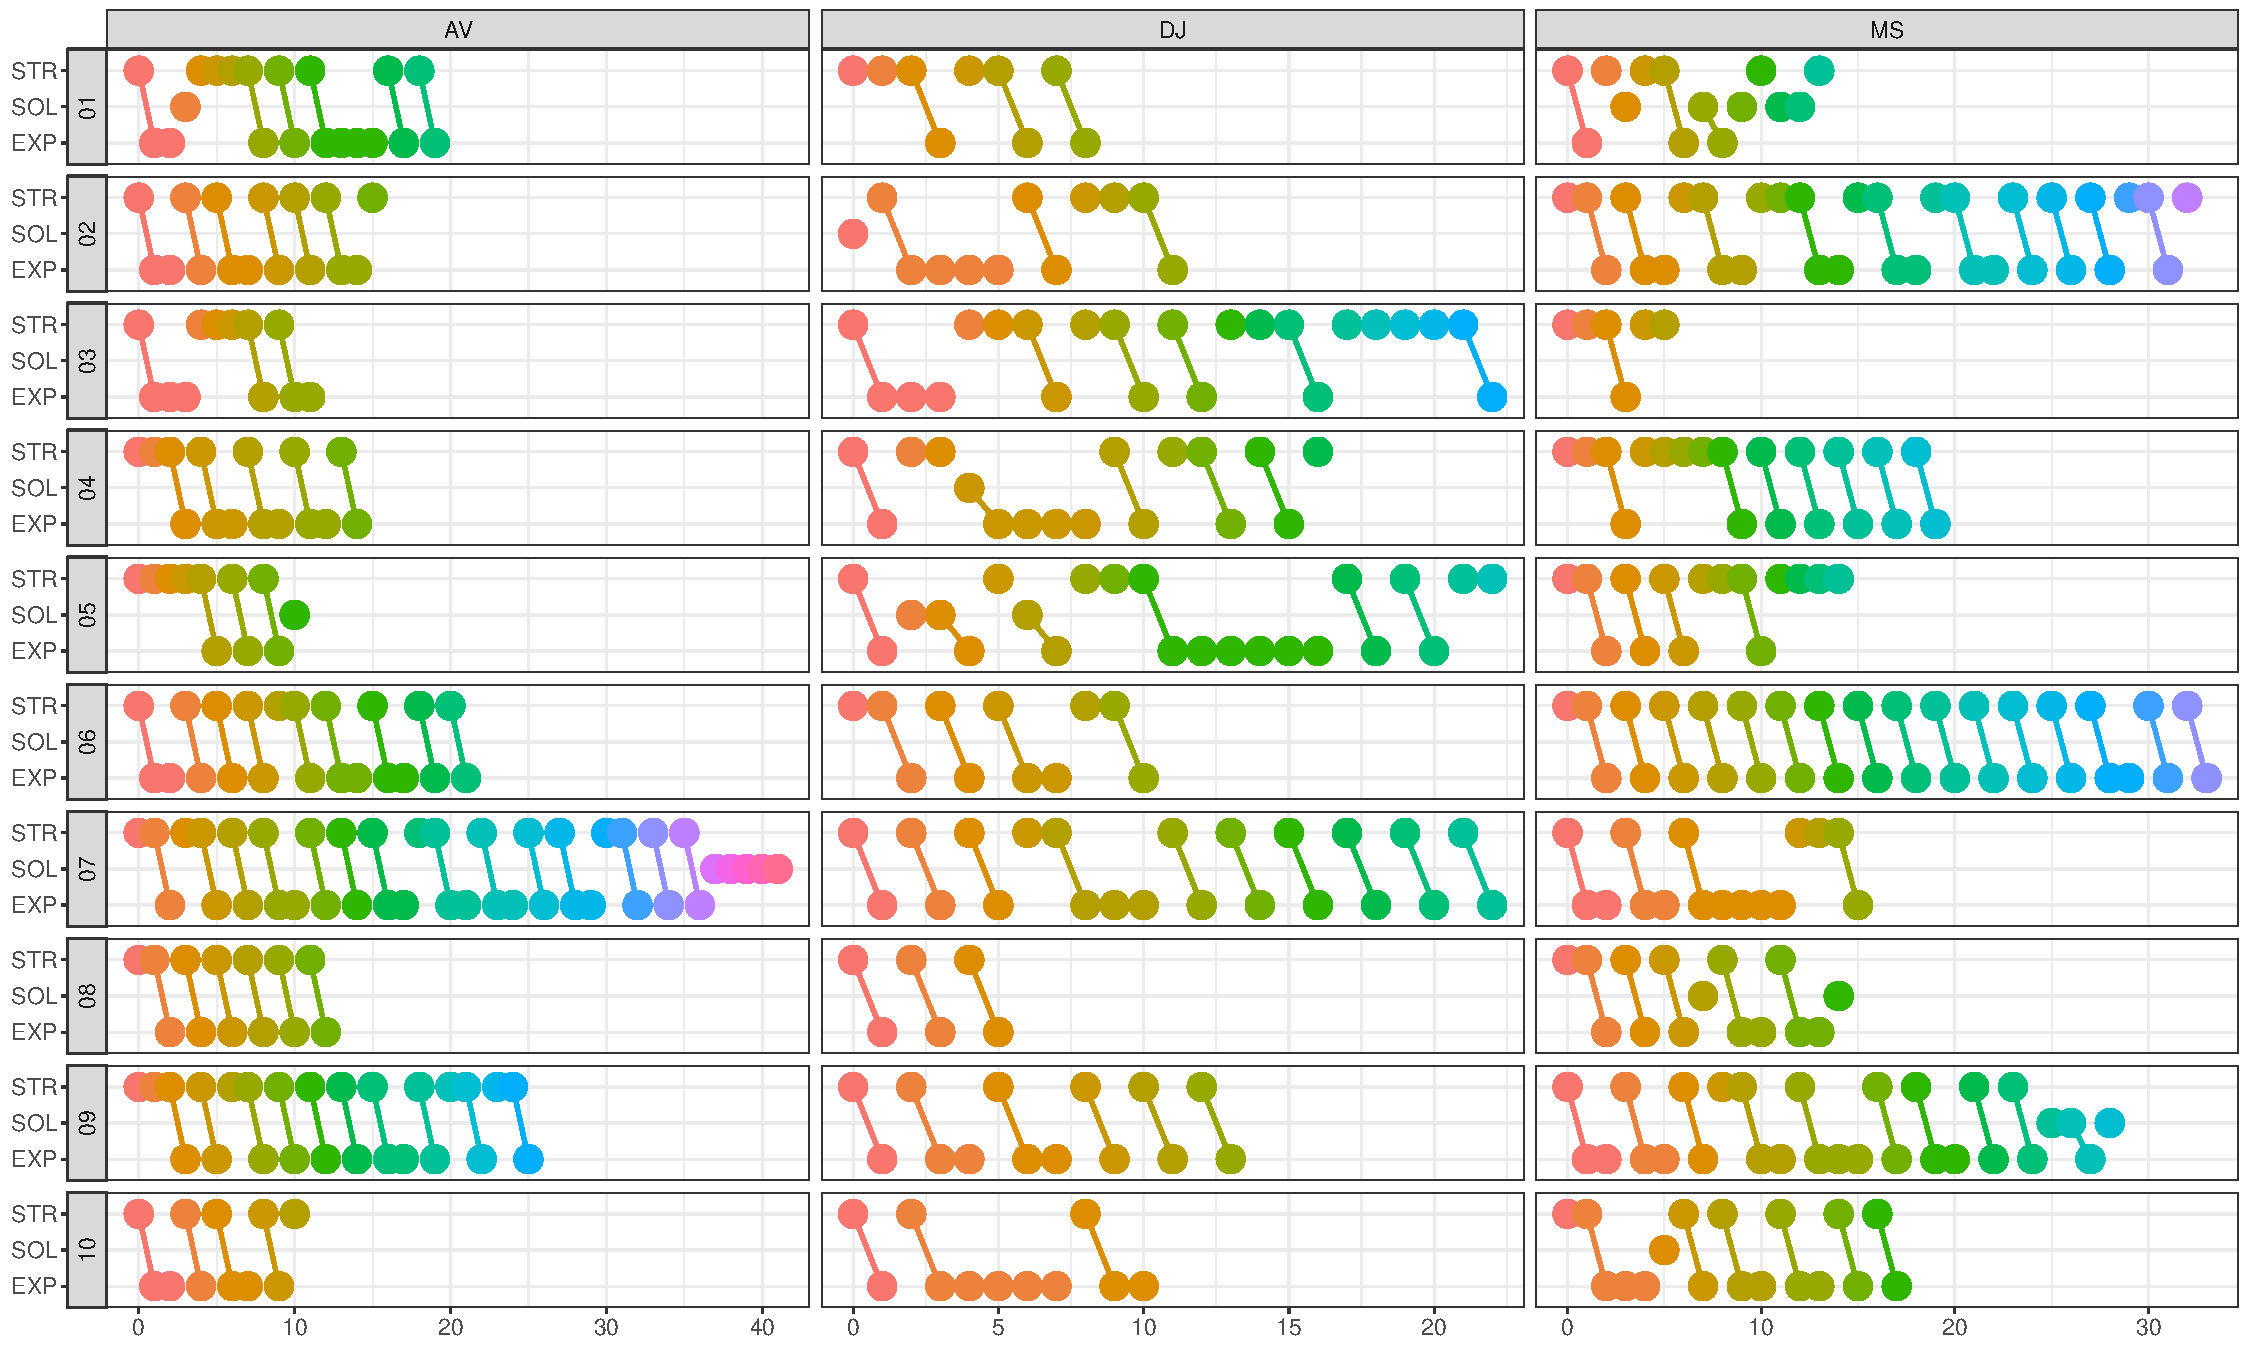
\includegraphics[width=\textwidth]{teachCyclesPltCombined}
\caption{Plot highlighting teaching cycles observed in collected explanation
artifacts. The y-axis is faceted to display the type of move for each coded
explanation. The x-axis indicates the position of a move within the
explanation. Connected sequences of dots represent a teaching cycle.}
\label{fig:cycles-plot}
\end{figure*}

\subsection{The Data}
\label{sec:exp:data}

We restrict the scope of data collection to include only objects that provide an
explanation of common computer science algorithms from computer
science departments at accredited universities. Restricting the scope of objects
in this manner provides two benefits: 1) All explanatory objects have a stated,
intrinsic goal to communicate the mechanics, application, or implementation of
some common computer science algorithm. 2) There are bountiful and varied
examples of different approaches to explain \emph{the same} algorithm, and numerous
examples of \emph{like} approaches to explain different algorithms.

All data was coded by hand by individuals (coders) with access to a reference
document specifying the typology. Explanatory objects were indexed according to
the algorithm that was to be explained, and a simple counter. For example, the
first document regarding AVL Trees would be named ``AVL001'' while the sixth
would be ``AVL006'' and so on. All of the data analyzed in this paper was
collected by a single researcher. 

If a document changed subject abruptly, or the algorithm of interest was
discussed in a middle section, the coder was instructed just code for the
algorithm and stop when the document changed focus. For example, if a fifty page
document started to discuss quicksort on page thirty-two after discussing
mergesort the data would only include codings for the first thirty-two pages of
that document. We made no effort to control for the length of any document and
the data was post-processed to normalize all position information to the
length of each document.

% Should I say more about the data pre-processing?
The data was pre-processed using R and Hadley Wickham's excellent ``dplyr''
library \cite{Dplyr}, for the complete code see
\url{https://github.com/lambda-land/XOPTypology_Paper}. In short, the
pre-processing consists of creating an ``index'' variable that denotes the order
a move was encoded in relation to each document considered e.g. an index of 1
means that move happened immediately, and sequentially, after the move indexed
at 0.

% explanations, ten explanations per algorithm and five explanations per algorithm
% per document type. Hence, there are 10 documents on Dijkstra's shortest
% path algorithm with five of those ten being power point documents and the other
% five being lecture notes. All samples were collected from the internet, see
% \url{https://github.com/lambda-land/XOPTypology_Paper} for list of all sources
% by algorithm. 

\section{Results}

In this section we present our findings. We make three major observations from
the data: First, we observe the presence of teaching cycles in static
explanatory objects. Secondly, we observe that the present typology's
shortcomings are a reflection of the nature of static documents. Lastly, we
observe that document type appears to be a correlative factor to
the nature and type of teaching cycles.


\subsection{Teaching Cycles}
\label{sec:res:cycles}

To graphically observe, and represent, teaching cycles we form a dot plot for
each coded document, with lines connecting pedagogical moves that make up the
teaching cycle, as shown in Fig.~\ref{fig:cycles-plot}.
%
Each dot is representative of a single pedagogical move. The y-axis is faceted to display
the Type of Move for each coded document. For example ``AVL001'', the first
coded document for AVL Trees, has 3 types of pedagogical moves: STR, SOL, EXP.
One may also observe that this document has 4 different types of teaching cycles
viz. ``STR EXP EXP'', ``SOL'', ``STR'' and ``STR EXP \ldots''. Documents
indexed 1 -- 5 inclusive, correspond to power point documents, documents index 6
-- 10, correspond to lecture notes documents (word, html, or pdf).

Due to modifications to Bellack et al's typology we observe six types
teaching cycles for static explanatory objects. These are shown in the table in
Fig.~\ref{fig:cycles-table}.


% \newcommand{\Freq}[1]{\ensuremath{\text{Freq}_\text{#1}}}
\newcommand{\Freq}[1]{\ensuremath{\text{Freq}_\text{#1}}}

% Don't know how you want to format this, perhaps we make a bar graph?
\begin{figure}
\centering\footnotesize
\begin{tabular}{rr|rr|l}
\multicolumn{2}{c}{Slides} &
\multicolumn{2}{c}{Notes} & \\
\multicolumn{1}{c}{$n$} & \multicolumn{1}{c}{\%} &
\multicolumn{1}{c}{$n$} & \multicolumn{1}{c}{\%}
  & \multicolumn{1}{l}{Teaching cycle} \\ \hline
65 & 44.8 & 21 & 14.9 & STR \\
 8 &  5.5 & 10 &  7.1 & SOL \\
49 & 33.8 & 78 & 55.3 & STR EXP \\
19 & 13.1 & 31 & 22.0 & STR EXP \ldots \\
 3 &  2.1 &  1 &  0.7 & SOL EXP \\
 1 &  0.7 &  0 &  0.0 & SOL EXP \ldots \\
% total teach cycle ppt observations: 145
% total teach cycle ppt observations: 141
\end{tabular}
\caption{Types and frequencies of teaching cycles found in explanation artifacts.}
\label{fig:cycles-table}
\end{figure}

\section{Discussion and Results}
In this section we summarize and interpret the results presented above. To
ensure transparency and openness, the reader may find all raw data, and any
post-processing scripts published online \url{https://github.com/lambda-land/XOPTypology_Paper}

\subsection{Observed Teaching Cycles}
As shown in Fig.~\ref{fig:cycles-plot}, and listed in
Fig.~\ref{fig:cycles-table}, we observe several types of teaching cycles.
Explanations in static documents adhere to a general pattern of an introductory
structuring (STR) move, followed by either a expositing (EXP). Very rarely an
explanation takes the form of teaching cycle that begins with a soliciting (SOL)
move. Some cycles were \emph{atomic} in that they were isolated to a single
pedagogical move. These cycles are coded as a single STR or SOL move and are
synonymous with a single EXP move i.e. the document sets the context for an
explanation and then concludes the explanation within one \emph{unit} of the
document viz. a single slide for power point documents, or a single statement
for lecture notes. It is unsurprising that such atomic moves are observed with
more frequency in power point presentations than lecture notes, given the
medium's form. The majority of STR EXP moves come from word or html (lecture
note) documents. Again, this is an anticipated result, as one would expect
explanations in these documents to make more short moves that correspond to a
single paragraph of thought or explanation.

\subsection{Observed Typological Deficiencies}
\label{sec:res:analysis}
Of particular note in our data is the \emph{absence} of any teaching cycle which
includes a responding (RES) or reacting (REA) move. Bellack et al's typology is
founded upon Wittgenstein's concept of a \emph{language game}. When applied to
discourse in the classroom such a foundation is easy to interpret. The lecturer
makes a move in the language game, and the pupil can then respond with a move of
their own. Bellack et al's typology captures the essence of this dynamic through
structuring, soliciting, responding and reacting moves. However, when applied to
a static document, the foundations of which the typology rest are brought into
conflict with the nature of the document. Simply put, observing a responding or
reacting move, \emph{in} a static document would be nonsensical because the
document has no way to participate in the language game. Our analysis concludes
this fact, as expected, viz. that the modified typology, when applied to static
documents, constitutes a category mistake regarding the foundations of the
typology from which it is based. This fact may also be observed in the very
modifications made to Bellack et al's typology. Such modifications \emph{were
  required} in order to \emph{be able to} apply the typology to static
explanatory objects.

We believe that such deficiencies are promising ground for the creation of an
DSL in the XOP paradigm. One which would allow a static document \emph{to
  participate} in a language game. The modified typology presented in this
paper serves as a scaffold or paradigm from which to design such a DSL in a
semantics-first \cite{EW11sle} manner.

\subsection{Observations While Encoding}
In general, the better structured the explanatory artifact, the easier it was to
encode. This observation is also represented in the data, namely in the number
of \emph{atomic} teaching cycles observed in a document. Documents which tend to
have a high amount of atomic teaching cycles were perceived to be more difficult
to encode, while documents that have an organizing internal structure were
perceived to be easier. Whether there is any pedagogical difference between the
two, or if this is just an artifact of a single coder, or an artifact of the
typology, is outside the scope of this paper, but the fact that such patterns
were observed does comport with Bellack et al.'s results. To be specific:

\say{With respect to the percentages of pedagogical moves, there seems to be
  little to differentiate the two groups --- with the exception, perhaps, of the
percentages of structuring moves. The range for the three classes judged
significantly high is very restricted (4.1 per cent to 5.2 per cent), but the
group judged significantly low includes both extremes of the range for all 15
classes (1.2 per cent and 13.2 per cent). This suggests that there may be an
optimum frequency for the use of the structuring move by the teacher as a way of
launching interaction between teacher and pupils and as a means of introducing
subject matter.}

\subsection{Applications to a DSL}
\label{sec:res:dsl}
An interactive DSL constructed in an XOP paradigm requires support for multiple
and varied notations, types of explanations, and different pacing of material,
all at the request or specification of the user. A typology of explanation can
serve as the basis, the backbone, of such a DSL by organizing the semantics of
the DSL into defined concepts. The modified typology presented in this paper, we
believe, serves as such an organizing tool. In this section we will discuss what
we believe the advantages are of designing around such a conceptual framework.

\subsubsection{The Usefulness of a Typology}
A DSL designed with the modified typology given above will have, as its
fundamental conceptual unit, a pedagogical move. Much like a DSL for displaying
graphics might have as its conceptual unit a Pixel. An explanation is then the
sequential composition of pedagogical moves into teaching cycles, that lead the
user from non-understanding, to understanding. The modified typology is
pragmatic for this domain \emph{because} of its level of abstraction. Each move
would be coded according to the counterpart categories in the typology. Thus,
the explanation for mergesort may require 15 moves, 5 teaching cycles. The
initiatory moves might be of the form ``STR/BKG/XPL'' or ``STR/MOT/VIS'',
meaning that the explanation would begin with a structuring move in which the
background of mergesort is explained, or a structuring move where the motivation
for mergesort is given visually. The pedagogical moves therefore structure the
semantics of the DSL by describing \emph{what the pedagogical move needs to
  accomplish and how}. It is because of the level of abstraction in the codes,
that concrete detailed aspects of explanations, like notation, or cadence become
liquid i.e. they become easy to change. Thus, by designing around a typology of
explanation, one ensures that the DSL has a defined pedagogical structure, but
is extensible, and not artificially constrained by the design.

\subsubsection{Structuring Explanations}
A secondary benefit of designing around a typology of explanation is that the
typology provides a rich tool for analyzing explanations in the wild from which
a language designer could draw a one-to-one plan from. For example, a document
explains an AVL tree data structure in twenty five moves and four teaching
cycles, an XOP DSL, could follow such a formula almost exactly because the
design was based on a typology of explanation. Such a ``harvesting of ideas'' is
simply not possible without a typology of explanation. One might even imagine a
program that scours the internet harvesting such explanations and creating a
corpus of explanations.

\subsubsection{Dealing with Notations}
An XOP DSL must be able to accommodate a multitude of notations. From
mathematics, to english, to visual notations and interactive diagrams. A DSL
designed in the manner above is extensible enough to support such
notations. For example, imagine a user who is unsatisfied with, or does not
understand a given pedagogical move, perhaps ``EXP/MAN/XPL'' (An expositing move
that is explaining the manipulation of something). What might the user do in such a
circumstance? In an XOP DSL, based on the modified typology, the user would be
able to request the same pedagogical move, given with a different notation. The move's
semantics would be the same: an expositing move that explains the
manipulation of the subject, but the notation may change from text, to a
diagram, to interactive illustrations freely. It is the ability to change the notation
that separates this approach with from previous strategies.

\subsubsection{Interactivity via Responding Moves}
A major result of the analysis of static artifacts given above was that,
unsurprisingly, static artifacts have no mechanism for a viewer to respond, they
are in not so many words, static. By designing a DSL according to a typology of
explanation one is able to provide a mechanism for responding or reacting moves
in some form. The typology forms the semantics of the DSL, and while the exact
mechanism to handle such prompts is unclear, a DSL designed in such a way has a
``hole'' in its structure for such a mechanism. One could easily imagine that
moving backward or forward in the explanation could be a primitive reacting
move. Similarly, the prompts to complete some question in many online tutorial
videos could be seen as a primitive soliciting move that is closed with a
responding move by the user. By designing with respect to the modified typology,
these concepts become clear, compartmentalized, and structured, in a way that is
not possible without a typology of explanation.

\subsubsection{Qualities shared with Passive Explanations}
Our approach differs from many other successful
approaches\cite{brecht2012learning, brecht2008enabling}, but shares many
important features of those approaches. Algorithm visualizations and internet
based lectures have the property of being random access i.e. the user may move
forward, backward, increase or decrease the pace, of the lecture at will. This
property has shown to be a very effective pedagogical tool\cite{cardall2008live,
  zhang2005interactive, zhang2006instructional, Schwan2004293, Merkt2011687} .
While such a property ultimately comes down to the implementation of the DSL, we
believe that our approach is commensurable with, and supportive of, such a
property. One could easily imagine the ability to proceed to the next
pedagogical move, return to the last pedagogical move or jump to an arbitrary
move in the explanation.

It is for the reasons stated above that we believe defining and employing
typologies of explanation provide the an explanation designer with invaluable
tools. Tools which serve to enrich the state of XOP and allow the explanation
designer to draw upon other domains to form their explanations.

\section{Related Work}
\label{sec:rw}

In this section we explore work that is related to this analysis and consider other
typologies from pedagogy scholarship.

\subsection{Algorithm Visualization}
\label{sec:rw:vis}

\todo{Algorithm visualizations target the same ``sweet spot'' we do but aren't
comprehensive.}

An \emph{algorithm visualization} is a graphical illustration, such as a
sequence of diagrams or an animation, of how an algorithm executes on given
inputs. As an example, consider the visualization in
Fig.~\ref{fig:negative-dijkstra}.


\todo{Move this figure and use it as an example of a \emph{negative} example,
which are not typically supported by algorithm visualizations.}

\begin{figure}
\centering
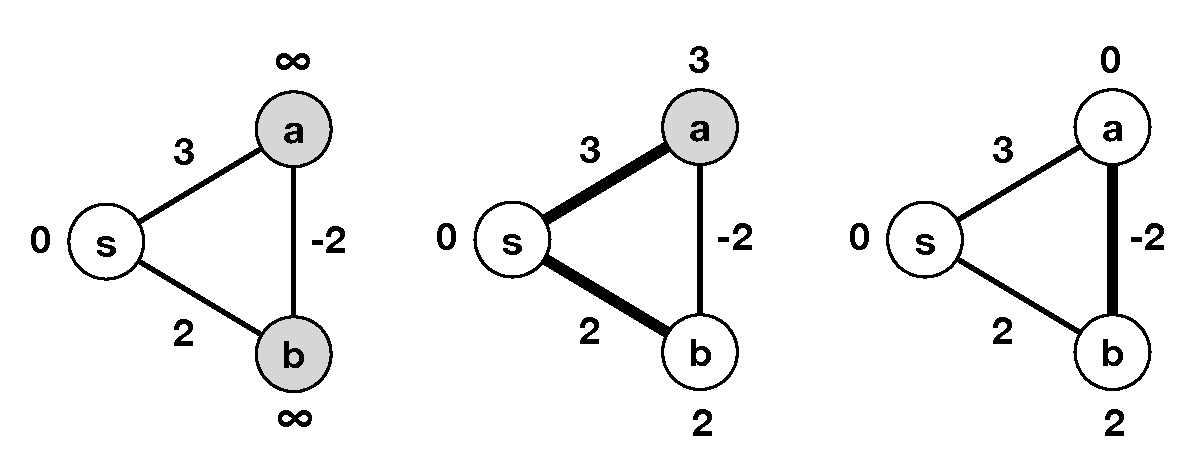
\includegraphics[width=0.9\columnwidth]{VisDJK010-Clean}
\caption{Example visualization of Dijkstra's algorithm failing on a graph with
negative edge weights. This is a (redrawn) visualization extracted from one of
the explanation artifacts in our data set (DJK010).}
\label{fig:negative-dijkstra}
\end{figure}


\todo{finish this paragraph}
\say{With few exceptions, we found that studies in which students merely viewed
visualizations did not demonstrate significant learning advantages over
students who used conventional learning materials.}
%
\cite{HDS02}.

Unfortunately, negative examples such as the one provided are not rare in
algorithm visualizations. Worse still many algorithm visualizations are not
maintained by a community or suffer from being too
simplistic\cite{shaffer2010algorithm} \todo{this may be another contribution,
  the DSL as a platform for cataloging Algorithm visualizations via a library system}

\subsection{Other Typologies of Explanation}
\label{sec:rw:typ}

Pedagogic theory has many examples of typologies of explanation which are not
presented here \cite{Smith1970-SMIASO-13, smith1967language, hyman1968teaching, swift1961explanation} . We adapt Bellack et al's because it is designed with the same
motivating research questions in mind as this work, namely quantifying
real-world examples of explanations. It also is \emph{computational} in nature
--- it adheres to a strict semantics and is rigorously, mathematically, defined.
In this section, we will briefly review alternative typologies and state our
reasons for not adapting them.

Brown and Armstrong\cite{brown1984explaining} developed a typology that sought
to qualify characteristics of \emph{good} explanations provided by teachers in a
classroom setting. Their typology was formed with two stated goals: 1) It should
be simple, elegant, and easy to pick up for student teachers and 2) It should be
powerful enough to characterize bad explanations from good ones, and relate to
previous pedagogic work. Their typology consists of ``keys'', which partition an
explanation, ``Links'' which form chains of keys that form the explanation, and
``Rules'' which define any pertinent rules to for that which is being explained.
There are three categories of explanation in the typology: 1) The Interpretative
2) The Descriptive and 3) The Reason Giving. While promising, the presentation
of this typology was deemed not formal enough to be actionable for our purposes;
for example, its presentation lacks definitions for significant terms such as
``Links'' and ``Rules''. Furthermore, its desirable features are shared with
Bellack et al's typology viz. an explanation is a composition of more
primitive concepts or categories.

%probably need an introductory sentence here
Roshenshine's\cite{rosenshine1968objectively} typology is generated through a
review of thirty lectures and the results of a user study. It's stated purpose
is to:

\say{objectively measure teaching behaviors that discriminate between more and
  less successful explanations of social studies material}. 

Rosenshine develops the grammar of terms based on a literature review of four
categories: 1) Linguistic Categories 2) Instructional Set 3) Presentational
categories and 4) Multivariate studies of teaching behaviors. Twenty one such
terms were identified and then tested in a user study for pedagogic impact. The
terms in the typology may include verbal and non-verbal behaviors in teachers.
While Rosenshines results were interesting the typology developed is
un-actionable for our purposes. The terms developed are either too broadly
defined, not translatable to a DSL, or by Rosenshines own research do not
correlate to a \emph{good} explanation. Furthermore, there is no set criteria
presented for encoding lectures with the typology. It is possible to adapt
Rosenshines work for our purposes but the resultant typology would differ so
radically from the original that it may no longer be relevant to Rosenshines own
work. Or to be succinct, Rosenshines typology is not easily extensible.

\section{Conclusion}

The conclusion goes here.


\section*{Acknowledgment}

The authors would like to thank...

\bibliography{XOPbib.bib,eric.bib}
\bibliographystyle{abbrv}

\end{document}
